\documentclass{standalone}
\usepackage{tikz}
\usetikzlibrary{patterns, angles}

\begin{document}
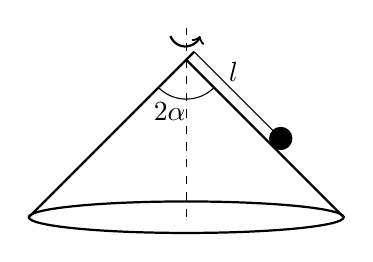
\begin{tikzpicture}
	\coordinate (A) at (-2, 0);
	\coordinate (B) at (0, 2.0);
	\coordinate (C) at (2, 0);
	
	\draw [thick] (0,0) ellipse (2 and 0.2);
	\draw [dashed] (0,0) -- (0,2.4);
	\draw [thick] (A) -- (B) -- (C);	
	\draw [thick, ->] (-0.2, 2.3) arc (200:340:0.2);
	\pic [draw, -, angle eccentricity=1.5] {angle = A--B--C};
	\node [left=6pt, below=12pt] at (B) {$2\alpha$};
	\draw [thick] (0,2) -- (0.1,2.1);
	\draw (1.1,1.1) -- (0.1,2.1) node [midway, above] {$l$};
	\draw [fill] (1.2,1.0) circle (0.141);
	
\end{tikzpicture}
\end{document}